% \documentclass[twoside,twocolumn]{ujarticle}
\documentclass[titlepage]{jarticle}
%\usepackage{type1cm}
\usepackage{outline-ec}
\usepackage{amsmath,amssymb,verbatim,ascmac,multicol}
\usepackage{tabularx}
% dvioutで確認する場合は以下を有効にする
%\usepackage[dviout]{graphicx,color}
% pdf化する場合は以下を有効にする
\usepackage[dvipdfmx]{graphicx,color}
%
% --------------------------------------------------------------------------
% 図表番号の後の:を削除
%
\makeatletter
\long\def\@makecaption#1#2{% #1=図表番号,#2=キャプション本文
\sbox\@tempboxa{#1 \hskip0.5zw #2}% 図表番号とキャプションの間のスペース 0.5zw
\ifdim \wd\@tempboxa >\hsize
#1 #2\par 
\else
\hb@xt@\hsize{\hfil\box\@tempboxa\hfil}
\fi}
\makeatother
% --------------------------------------------------------------------------

%
% --------------------------------------------------------------------------
% 下の該当する部分を書き換える
%
\氏名{本間 三暉}			%% 自分の氏名
\出席番号{35}					%% 出席番号
\研究室名{視覚情報処理研究室}			%% 研究室名
\指導教官{高橋 章}			%% 指導教員名
%
% --------------------------------------------------------------------------
% 研究題目等
%
% 研究題目が2行になるときは \\ で行送りできる
%
\発表番号{B\;--\;}
\研究題目{単一視点による人物の三次元動作解析について}

% --------------------------------------------------------------------------
% アブストラクト
%
\アブストラクト{
複数のRGBカメラやモーションキャプチャなどの専用のデバイスでは,予算の都合などから動作推定できない場合がある.これに対し,運動を行う人物を一台のRGBカメラやRGBDカメラで撮影し,それぞれのカメラに合った画像処理を用いた手法で三次元骨格推定を行う.
それらの方法で行った三次元骨格推定の結果を精度や処理速度などについて比較し分析する.
% また,組み込みPCで実装する場合やカメラに対し手前にある物体が後ろにある物体を隠す状態になり十分に計測できないオクルージョンへの対応,
% リアルタイム処理を目的とした高速化を目指す.
% =======
% モーションキャプチャデバイスmocopiでは表現しきれない部分を画像処理を用いて補助することを検討する.
% mocopiでは関節部などが正確に計測できないことがあるため,竹馬や一輪車などの精密な重心移動や姿勢制御が必要な運動に関して測定を行い,
% 画像処理による骨格推定を組み合わせ,バランス運動時の重心や姿勢を解析することによって,mocopiの測定精度を上げることを目指す.
}
%
% --------------------------------------------------------------------------
% 本文開始
%
\begin{document}
\maketitle

%
% --------------------------------------------------------------------------
% 第1節
%
\section{研究背景・目的}
%
情報通信技術の急速な進歩により人工現実感,拡張現実感,複合現実感などの応用が広がっている.
感染症対策を契機にオンラインコミュニケーションも増加し,インターネット上の仮想共有空間であるメタバースが注目されている.\cite{meta}
その理由の一つに,離れている相手にテキストや音声だけでなく身振りや動作などのノンバーバルな情報の伝達を行うことが容易であるという点がある.
三次元の仮想空間で自分の分身となるアバターを自由に操作するには,
体の動きを計測する必要があり,画像処理による方法\cite{CV}や専用デバイスを装着する方法\cite{キャプチャ}などが試みられている.
画像処理による方法で三次元の情報を取得するためには先行研究のような複数台のカメラを用いる方法\cite{turugi}があるが,狭い室内であるなどの場所の制約や,
限られた予算の中で実装したいという資金の制約などによって,複数台のカメラを用いる方法取るのが難しい場合がある.

本研究では1台の入力装置で三次元骨格推定ができる現行の方法について実験を行い,それぞれの方法のメリットやデメリット,精度などについて比較する.
また,それらの情報を元に組み込みPCでの実装やリアルタイム処理などの高速化,オクルージョンというカメラに対し手前にある物体が後ろにある物体を隠す状態になり十分に計測できない場合への対応を目指す.

% 情報通信技術の急速な進歩により人工現実感,拡張
% 現実感,複合現実感などの応用が広がっている.感染
% 症対策を契機にオンラインコミュニケーションも増加
% し,インターネット上の仮想共有空間であるメタバー
% スが注目されている.メタバースが注目されている理
% 由の一つに,離れている相手にテキストや音声だけで
% なく身振りや動作などのノンバーバルな情報の伝達
% を行うことが容易であるという点がある.三次元の仮
% 想空間で自分の分身となるアバターを自由に操作する
% には,体の動きを計測する必要があり,画像処理によ
% る方法 [1] や専用デバイスを装着する方法 [2] などが試
% みられている.画像処理による方法で三次元の情報を
% 取得するためには先行研究のような複数台のカメラを
% 用いる方法 [3] があるが,狭い室内であるなどの場所
% の制約や,限られた予算の中で実装したいという資金
% の制約などによって,複数台のカメラを用いる方法や
% 専用デバイスを装着する方法を取るのが難しい場合が
% ある.
% 本研究ではカメラ 1 台で三次元骨格推定ができる
% 現行の方法について実験を行い,それぞれの方法のメ
% リットやデメリット,精度などについて比較する.ま
% た,それらを元に組み込み PC での実装やリアルタイ
% ム処理などの高速化,オクルージョンというカメラに
% 対し手前にある物体が後ろにある物体を隠す状態にな
% り十分に計測できない場合への対応を目指す.

% 本研究では市販のモーションキャプチャデバイスmocopiを,運動解析に活用することを検討する.
% このデバイスは両手,両足,頭,腰の計6か所に小型センサを装着してリアルタイムに三次元計測を行うことができるが,肘や膝などの関節の屈曲を正確に計測することができない.
% そこで画像処理による骨格推定を組み合わせ,一輪車や竹馬のような器具を使うバランス運動の動作解析を実現する.
% これにより,身体が身体自信や使用器具などに隠れてしまう場合の骨格推定の精度低下の解消,三次元計測の精度の向上,計測速度のさらなる改善などの問題を解決することが出来る.
% そして、スポーツや映像作品などの様々な分野で,使い方が限定されていたモーションキャプチャの応用範囲が広がることが期待できる.
%
% --------------------------------------------------------------------------
% 第2節
%
\section{研究内容}
%これって研究背景に描いたほうが自然か?

%
% --------------------------------------------------------------------------
% 第2節 第1小節
%
\subsection{人の動作の計測方法}
%
人の動作の三次元計測を行うには,画像処理による方法やモーションセンサによる方法などがある.それぞれの方法について簡単にまとめたものを表\ref{3D_1}に示す.
画像処理による方法では画像から人の骨格を推定することで人の動作を解析できる.
画像処理による三次元骨格推定は撮影するカメラに,色情報を記録できる一般的なRGBカメラを用いて解析する方法と,
カメラと物体の距離を測ることができるRGBDカメラ用いて解析する方法がある.
% これらの方法はモーションセンサを用いるものと比べると精度にばらつきが生まれる.

%% モーションセンサのしゅるいについてもかいたほうが自然か?
% モーションセンサによる方法は光学式や慣性式などがあるが,どの方法も精度が高いかわりにマーカーやセンサを検出対象に取り付けなければならないため使用できる環境が限定されてしまう.
モーションセンサによる方法は,光学式や慣性式などがある.
光学式は体中にマーカーを取り付けそのマーカーを複数台のカメラで取り込むことで,
慣性式は加速度,角速度,方位を測定できるセンサを体中に取り付けることで骨格を推定する.

\begin{table}[t!]
  \centering
  \caption{動作を計測する方法の種類と特徴}
  \begin{tabular}{l|ll|ll}
    \hline
          & \multicolumn{2}{c|}{カメラ}       & \multicolumn{2}{c}{モーションセンサ}                                  \\ \cline{2-5}
          & \multicolumn{1}{l|}{RGB}       & RGBD                         & \multicolumn{1}{l|}{光学式} & 慣性式 \\ \hline
    センサ装着 & \multicolumn{1}{l|}{不要}        & 不要                           & \multicolumn{1}{l|}{必要}  & 必要  \\
    外から撮影 & \multicolumn{1}{l|}{必要}        & 必要                           & \multicolumn{1}{l|}{必要}  & 不要  \\
    必要台数  & \multicolumn{1}{l|}{1$\sim$数台} & 1台                           & \multicolumn{1}{l|}{複数}  & 0   \\ \hline
  \end{tabular}
  \label{3D_1}
\end{table}

% 動作人の動作の三次元計測を行うには,画像処理に
% よる方法やモーションセンサによる方法などがある.
% 画像処理による方法では画像から人の骨格を推定する
% ことで人の動作を解析することができる.画像処理に
% よって三次元骨格推定するには,撮影するカメラに色
% 情報を記録する一般的な RGB カメラで撮影して解析
% する方法と,kinect や RealSense のようなカメラと物
% 体の距離を測ることができる RGBD カメラで撮影し
% て解析する方法がある.モーションセンサによる方法
% は光学式や慣性式などがあるが,どの方法もマーカー
% やセンサを検出対象に取り付けなければならないため
% 使用できる環境が限定されてしまう.
% 本研究では場所や資金の制約があるような場面に対
% 応できるように,一台のカメラと画像処理により三次
% 元計測を行う場合の方法について検証する.

本研究では一台のカメラと画像処理で三次元計測を行う場合について検証し,モーションセンサを用いて三次元測定した場合と比較する.
% 今回は場所や資金などの制約から一台のカメラで人の動作の三次元計測を行う場合に限定して比較するので,
% 先行研究\cite{turugi}のような複数台のカメラを用いて三次元計測を行う場合を除いた方法について検証する.

%
% --------------------------------------------------------------------------
% 第2節 第2小節
%
\subsection{RGBカメラ一台を用いた三次元骨格推定}
%
RGBカメラで撮影して推定する方法では処理に3d-pose-baseline\cite{baseline}とOpenPose\cite{openpose}を用いる.

OpenPoseは,人体の18個のキーポイント(関節)とその関節をつなぐボーン(骨)を検出することができるオープンソースである.
OpenPoseは,正面からの画像だけでなく横からでも姿勢推定を行うことができる.
また,信頼度は低下するが遮蔽物により,見えない部位の推定も行うことができる.

3d-pose-baselineは,三次元の姿勢情報と二次元に投影した姿勢情報を機械学習することで,
二次元の姿勢推定情報から三次元の骨格推定が行え,その座標情報を取得できるオープンソースである.

RGBカメラ一台と画像処理から三次元骨格推定を行う\cite{ビデオ}流れを図にまとめたものを図\ref{RGB}に示す.
% \begin{enumerate}
%   \item 2000万画素,30fpsのGoProで運動している人物を撮影
%   \item 撮影した動画を連続静止画へ変換
%   \item 各静止画からOpenPoseで関節の二次元位置を抽出
%   \item 関節の二次元位置を時間軸方向に平滑化
%   \item 関節の二次元位置を3d-pose-baselineの入力形式に変換
%   \item 3d-pose-baselineで三次元位置を推定
% \end{enumerate}

\begin{figure}[b!]
  \centering
  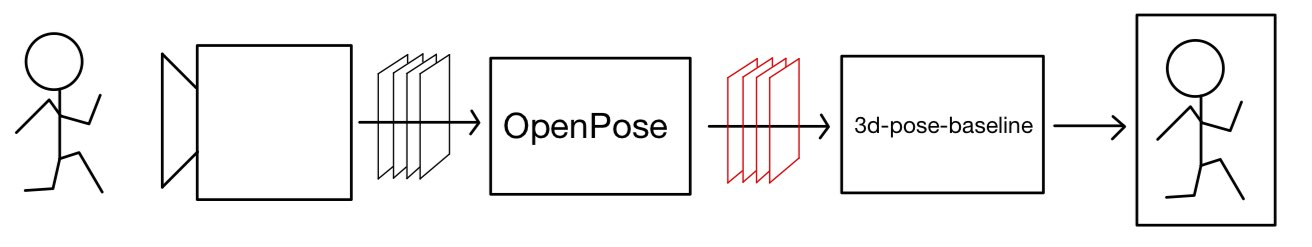
\includegraphics[width=6cm]{img/RGBcamera.jpg}
  \caption{単一RGBカメラによる三次元骨格推定の流れ}
  \label{RGB}
\end{figure}

RGBカメラで運動している人物の動作を撮影し,その動画を連続静止画へ変換する.各静止画からOpenPoseで関節の二次元位置を抽出する.

抽出した各点の二次元位置を三点移動平均など用いて時間軸方向に滑らかな動作をしているように.
そうして動きを滑らかにした関節の二次元位置を3d-pose-baselineの入力形式に変換し,3d-pose-baselineを用いて三次元位置を推定する.

\subsection{RGBDカメラで行う三次元骨格推定}
入力を
% kinect2やintelのRealSenseなどの
RGBDカメラにする場合,kinectSDK\cite{kinectSDK}などのハードウェアの公式から出ているソフトウェアやmediapipe\cite{cubemos}などのオープンソースを処理に用いることによって三次元骨格推定を行うことができる.
RGBDカメラと開発ライブラリの組み合わせを表\ref{RGBD}に示す.
\begin{table}[t!]
  \centering
  \caption{RGBDカメラと開発ライブラリの組み合わせ}
  \begin{tabular}{l|l}\hline
    カメラ       & ライブラリ            \\\hline
    kinect2   & kinectSDK,OpenNI \\
    RealSense & mediapipe        \\\hline
  \end{tabular}
  \label{RGBD}
\end{table}

kinectSDKはMicrosoft Kinect for Windows Software Development Kit の略で,Microsoft社から公式にリリースされた開発キットである.
Windows上でkinect2を動かすのに必要なドライバやドキュメントなどが同梱されていて,ソフトウェアであるkinectSDKとハードウェアであるkinect2があれば最低限動く様になっているが,
現在は開発が終了してしまっている.

kinectSDKと似たような機能を持つもので,Kinectのセンサ部分を開発したPrimeSense社が中心となって開発したOpenNIというライブラリがある.
OpenNIの構成を図\ref{app}に示す.
OpenNIには部分的なトラッキングやジェスチャ検出機能などkinectSDKに比べできることが多く,GitHub上でソースコードが公開されており現在も有志による開発が行われているが,
OpenNI自体はミドルウェアの位置付けでありアプリケーションとハードウェアの架け橋に過ぎないのでこれだけで動くことはない.

\begin{figure}[b!]
  \centering
  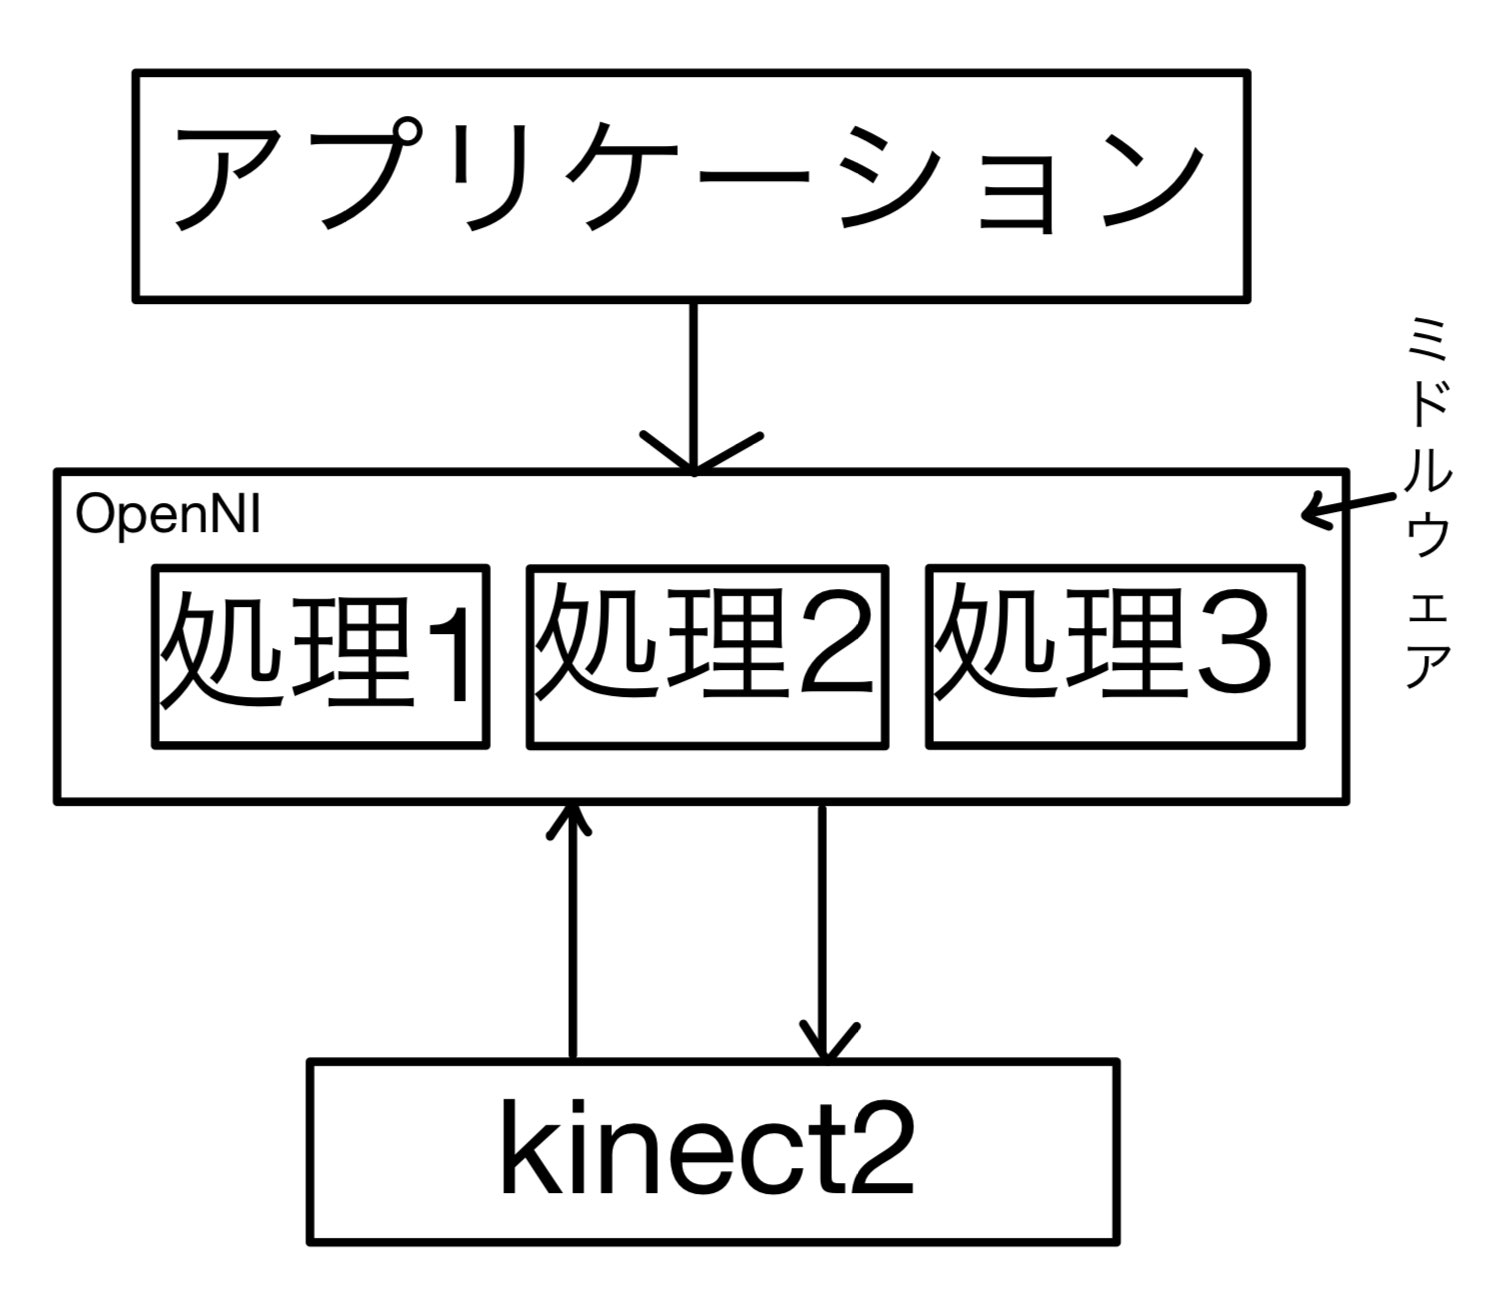
\includegraphics[width=6cm]{img/app1.jpg}
  \caption{OpenNIの構成}
  \label{app}
\end{figure}


% kinect2で撮影する場合はkinectSDKやOpenNIを用いて解析することで三次元骨格推定を行うことができるが,kinectSDKとOpenNIの両方に長所と短所があるためそれぞれの場合について実装し比較を行う.

mediapipeはGoogleが提供しているライブメディアやストリーミングメディア向けの機械学習ソリューションである.
特徴として,少ない記述量で使う事ができて,バッテリー駆動のデバイスでも十分に動作するよう設計されているというものが挙げられる.

% RealSenseで撮影する際,medeiapipeのPoseを使うことによって三次元骨格推定をすることができる.

% kinectSDKを使うことでkinect2に搭載されているセンサを制御してRGB画像や奥行き情報をPCに入力することができる.
% また,それらの情報から人体の骨格を自動的に検出し,その骨格を追跡することができる.

% kinectSDKとはMicrosoft Kinect for Windows Software Development Kit の略で,Microsoft社から公式にリリースされた開発キットで,
% Windows上でkinectを動かすのに必要なドライバやドキュメントなどが同梱されている.

% 似たような機能を持つもので,Kinectのセンサ部分を開発したPrimeSense社が中心となって開発したOpenNIというライブラリがある.
% こちらには部分的なトラッキングやジェスチャ検出機能などkinectSDKに比べできることが多く,GitHub上でソースコードが公開されており現在も有志による開発が行われているが,ドライバが同梱されておらず一つのライブラリで完結しないという欠点がある.
% kinectSDKは現在開発が終了してしまっているので,どちらにも長所と短所が存在する.%%
% kinect2で撮影する場合はkinektSDKやOpenNIを用いて解析することで三次元骨格推定を行うことができる.

%% cubemosのSkeleton Tracking SDKもう使えないマ?
% RealSenseを用いる方法では,cubemosのSkeleton Tracking SDK\cite{cubemos}を使うことによって三次元骨格推定をすることができる.
% cubemosのSkeleton Tracking SDKはディープラーニングベースの2D/3D骨格トラッキング機能を,組み込みハードウェア向けのアプリケーションへ提供するよう設計されたソフトウェアである.
% そのため,GPUがなくても動き,WindowsやLinux上で動かせ,対応言語が比較的多いという特徴がある.
%
% --------------------------------------------------------------------------
% 第2節 第3小節
%
% \subsection{}
%

%
% --------------------------------------------------------------------------
% 第2節 第4小節
%
\subsection{画像処理データの比較方法}
%
各画像処理の精度を比較する際,画像処理による方法で取得したデータを基準にするのは特定の骨格推定の方法に有利な結果が出てしまう可能性があるため,基準とするデータは画像処理に頼らない独立した方法で行う必要がある.
また,人体の左右対称性を考慮した骨格データが出てくるなどの理由からモーションキャプチャデバイスmocopi\cite{mocopi}を用いる.

% 現行のRGBカメラやRGBDカメラで同時に撮影し処理を行うような方法を比較する際,
% 画像処理による方法で取得したデータを基準にするのは特定の骨格推定の方法に有利な結果が出てしまう可能性がある.そのため,基準とするデータは画像処理に頼らない独立した方法で行う必要がある.
% また,人体の左右対称性を考慮した骨格データが出てくることなどがmocopiを用いる理由である.

mocopiとは,市販のモーションキャプチャデバイスで両手,両足,頭,腰の計6か所に小型センサを装着してリアルタイムに三次元計測を行うことができる.
6つの小型センサで測定しているため肘や膝などの関節部の屈曲を正確に表現することはできないが,mocopiのセンサはそれぞれ3つの自由度を持つ加速度センサと角度センサで測定しており,
機械学習を用いることで,肘や膝などの関節部を含めた全身の推定を実現している.

% mocopiとは,市販のモーションキャプチャデバイスで両手,両足,頭,腰の計6か所に小型センサを装着してリアルタイムに三次元計測を行うことができる.
% mocopiのセンサはそれぞれ3つの自由度を持つ加速度センサと角度センサで測定しており,AIを利用して人の様々な動作を予め学習させておくことで,センサを装着していない肘や膝などの中間関節を含めた全身の推定を実現している.
% よってmocopiでは肘や膝などの関節の屈曲を正確に表現することはできなが

% 加速度センサと角度センサが搭載されているモーションキャプチャデバイスmocopiを用いて取得した骨格データとの誤差を元に精度を比較する.
% 理由として,現行のRGBカメラやRGBDカメラで撮影し処理を行うような方法を比較する際,画像処理による方法で取得したデータを基準にするのは特定の骨格推定の方法に有利な結果が出てしまう可能性があり,
% 基準とするデータは画像処理に頼らない独立した方法で行う必要があるためである.

本研究では,学校体操やラジオ体操のような全身運動をしている人物一人に対して計測を行い,
mocopiのセンサの位置に当たる両手,両足,頭,腰の計6か所に関して,画像処理を用いて行った三次元骨格推定で得られた座標との誤差や時間変動を比較することで精度を評価する.
%
% --------------------------------------------------------------------------
% 第2節 第5小節
%
% \subsection{}
%

%
%
%
% --------------------------------------------------------------------------
% 第2節 第6小節
%
%\subsection{}
%

%
%
%
% --------------------------------------------------------------------------
% 第3節
%
\section{研究計画と進捗状況}
%

%
% --------------------------------------------------------------------------
% 第3節 第1小節
%
% \subsection{研究の進め方}
%
% mocopiを装着して学校体操をしている人をRGBカメラ,kinect2,RealSenseで同時に撮影する.
% それぞれのカメラで撮影した映像から三次元骨格推定を行い,推定した骨格とmocopiで測定した骨格の両手,両足,頭,腰の座標のズレを誤差として精度の計測を行う.

%
%
% --------------------------------------------------------------------------
% 第3節 第2小節
%
% \subsection{研究方法や装置の概略}
%
% ・撮影機材や開発環境について記述
% 本研究では,開発環境としてmocopiとOpenPoseを使用する.

% mocopi\cite{mocopi}とは,市販のモーションキャプチャデバイスで両手,両足,頭,腰の計6か所に小型センサを装着してリアルタイムに三次元計測を行うことができる.
% mocopiのセンサはそれぞれ3つの自由度を持つ加速度センサと角度センサ
現在は,OpenPoseによる姿勢推定を進めている.
今後はRGBカメラによる方法の他にRealSenseで撮影した動画から三次元骨格推定を行う測定プログラムをSDKやライブラリを用いて開発し,mocopiから得られた骨格データと比較分析する.
%
% ・mokopiに付いて記述
%


%
%
% --------------------------------------------------------------------------
% 第3節 第3小節
%
% \subsection{進捗状況}
%
% 現在は,OpenPoseによる姿勢推定を進めている.今後は記述した方法だけでなく,他にも単一のカメラで三次元骨格推定ができる方法がないかリサーチしつつ,オクルージョンへの対応,高速化,組み込みPCでの実装を目指していく.
%
% --------------------------------------------------------------------------
% 第3節 第4小節
%
%\subsection{}
%

%

%
%
% --------------------------------------------------------------------------
% 第3節
%
% \section{まとめと今後の予定}
%

% 学校体操や空手の型などの,体を大きく動かし,関節の位置や体の相対関係が正しく測定できるようにする.
%
% --------------------------------------------------------------------------
% 参考文献
%

\begin{thebibliography}{99}
  \small{
    \bibitem{meta}{
      日本経済新聞,``孤独感抱える若者の交流の場,メタバースに開設'',https://onl.la/Y7BehPP
    }
    \bibitem{CV}{
      平尾 公男ら,``多関節 CG モデルと距離画像による上半身の姿勢推定'',Technical report of IEICE.
      PRMU, VOL.104, No.573, 79-84, 2004.
    }
    \bibitem{キャプチャ}{
      白鳥 貴亮ら,``モーションキャプチャと音楽情報を用いた舞踊動作解析手法'',電子情報通信学会論文誌D,Vol.J88-D2,No.8,pp.1662-1671,2005.
    }
    \bibitem{turugi}{
      剱 一輝,``柔道競技の3Dアーカイブ化'',令和4年度長岡高専専攻科論文,2023.
    }
    \bibitem{baseline}{
      J. Martinez, R. Hossain, J. Romero, J. Little. ``A simple
      yet effective baseline for 3d human pose estimation'' . In
      ICCV, 2017.
    }
    \bibitem{ビデオ}{
      安達 康平ら,``ビデオからの3次元姿勢を用いた行動認識における精度向上の試み'',研究報告モバイルコンピューティングとパーベイシブシステム(MBL),
      2020-MBL-94,47,1-7,2020.
    }
    \bibitem{kinectSDK}{
      谷尻 豊寿,``体の動きがコントローラ C++でkinectプログラミング KINECTセンサ画像処理プログラミング'',株式会社 カットシステム,2011.
    }
    \bibitem{cubemos}{
      Google,``mediapipe'',https://developers.google.com/mediapipe
    }
    \bibitem{mocopi}{
      SONY,``モバイルモーションキャプチャーmocopi'',https://www.sony.jp/mocopi/
    }
    \bibitem{openpose}{
      CAO,Zhe,et al.OpenPose: Realtime Multi-Person 2D Pose Estimation Using Part Affinity Fields. arXiv preprint arXiv:1812.08008. 2018.
    }
  }
\end{thebibliography}
\end{document}
